\documentclass[review]{elsarticle}


\usepackage{graphicx}
\usepackage{amsmath}

\usepackage{subcaption}

\usepackage{amssymb}
\usepackage{array}

\usepackage{lineno,hyperref}
\modulolinenumbers[5]

%\usepackage{numcompress}\bibliographystyle{model3-num-names}

\usepackage{natbib}
%\usepackage[numbers, sort&compress]{natbib}
%\setcitestyle{author[oxford]year}
\bibliographystyle{elsarticle-num}

%\geometry{verbose,tmargin=30mm,bmargin=25mm,lmargin=25mm,rmargin=25mm}
%\newcommand{\templatefigures}[1]
{\noindent
\begin{minipage}{2cm}
\begin{center}
%\linespread{1}
%\begin{figure}
  \centering
	\vspace{-1cm}
  
\includegraphics[height = 63px]{ISI2019only_with_date_small.pdf}\\
    %\label{matrix}
%\end{figure}
\end{center}
\end{minipage}
%
\quad
%
\begin{minipage}{12cm}
\hspace*{6.8cm}
\end{minipage}
%
\quad
%
\begin{minipage}{2cm}
\begin{center}
%\linespread{1}
\vspace{-0.9cm}

\includegraphics[scale=0.4]{imag2.jpg}\\
\end{center}

\end{minipage}

\vskip0.2cm
}


%\pagestyle{empty}
\begin{document}
%\templatefigures{}




% Model ensembles with different response variables for base and meta models:



% Spatial and Spatio-temporal Epidemiology
% Special issue: Disease Surveillance and Infectious disease Modeling


\begin{frontmatter}

\title{Improving disaggregation models of malaria incidence by ensembling non-linear models of prevalence}

\author[oxford]{Tim C. D. Lucas\corref{mycorrespondingauthor}}
\cortext[mycorrespondingauthor]{Corresponding author}
\ead{timcdlucas@gmail.com}
\author[oxford]{Anita K. Nandi}
\author[oxford]{Emma L. Collins}
\author[oxford]{Suzanne H. Keddie}
\author[oxford]{Katherine A. Twohig}
\author[oxford]{Elisabeth G. Chestnutt}
\author[oxford]{Rosalind E. Howes}
\author[oxford]{Michele Nguyen}
\author[oxford]{Susan F. Rumisha}
\author[oxford]{Andre Python}
\author[oxford]{Rohan Arambepola}
\author[oxford,idm]{Amelia Bertozzi-Villa}
\author[oxford]{Penelope Hancock}
\author[oxford]{Punam Amratia}
\author[oxford]{Katherine E. Battle}
\author[oxford]{Ewan Cameron}
\author[oxford,telethon,curtin]{Peter W. Gething}
\author[oxford]{Daniel J. Weiss}



\address[oxford]{Malaria Atlas Project, Big Data Institute, University of Oxford, Oxford, UK}
\address[idm]{Institute for Disease Modeling, Bellevue, WA, USA}
\address[telethon]{Telethon Kids Institute, Perth Children’s Hospital, Perth, Australia}
\address[curtin]{Curtin University, Perth, Australia}



\begin{abstract}

Maps of infection rate are one of the core tools needed for the control and elimination of malaria.
As reliable routine surveillance data of malaria incidence becomes more widely available disaggregation regression is becoming an important model framework.
However, the aggregation of incidence over large, heterogeneous areas means that they are underpowered for learning complex, non-linear relationships between the environment and malaria risk.
In contrast, prevalence point-surveys are directly linked to local environmental conditions but are not common in many areas of the world.
A model that combines point surveys and aggregated surveillance data could have the benefits of both but must be able to account for the fact that these two data types measure different malariometric units.
Here, we train multiple non-linear, machine learning models on prevalence point-surveys.
We then ensemble the predictions from these machine learning models with a geostatistical disaggregation regression model that uses malaria incidence, aggregated to admnistrative units, as response data.
We find that, in four national case studies, using a disaggregation regression model to combine predictions from machine learning models trained on prevalence point-surveys improves model accuracy relative to a baseline disaggregation regression model that uses linear effects of the environmental covariates only.                                  

\end{abstract}

\begin{keyword}
Spatial statistics; Disaggregation regression; Stacking; Surveillance data
\end{keyword}

\end{frontmatter}

\linenumbers



\section{Introduction}


% New plan

% We need to do disaggregation but how do we do nonlinear

% We can do machine learning on prevalence and then combine...

% Stacking is a thing and has some nice theory.

% We found that it worked ok.


High-resolution maps of malaria risk are vital for control and elimination \citep{weiss2019mapping, battle2019mapping}.
However, mapping malaria in lower burden countries presents new challenges as traditional mapping of prevalence from cluster-level surveys \citep{weiss2019mapping,battle2019mapping, bhatt2017improved, bhatt2015effect} is often not effective for two reasons.
Firstly, so few individuals are infected that most surveys will detect zero cases \citep{sturrock2016mapping}.
Secondly, there is a lack of nationally representative prevalence surveys in low burden countries \citep{sturrock2016mapping, sturrock2014fine}. 
Routine surveillance data of malaria case counts, often aggregated over administrative regions defined by geographic polygons, is becoming more reliable and more widely available \citep{sturrock2016mapping} and recent work has focussed on methods for estimating high-resolution malaria risk from these data \citep{sturrock2014fine, wilson2017pointless, law2018variational, taylor2017continuous, li2012log}. 
However, the aggregation of cases over space means that the data may be spatially uninformative, especially if the case counts are aggregated over large or heterogeneous areas, because it is unclear where within the polygon, and in which environments, the cases occurred. 
This data is therefore often under-powered for fitting flexible, non-linear models as is required for accurate malaria maps \citep{bhatt2017improved, bhatt2015effect}. 
A model that combines prevalence point-surveys and aggregated surveillance data, and therefore leverages the strength of both, has great potential.

Here we propose training a suite of machine learning models on point-level, binomial prevalence data and combining these predictions by using them as covariates in a polygon-level, disaggregation regression model that uses  malaria incidence, aggregated to administrative units, as the response.
This modelling scheme has similarities to previous stacking methods used for malaria mapping \citep{bhatt2017improved} and elsewhere \citep{wolpert1992stacked, sill2009feature, hao2019review, breiman1996stacked}.
However, as the response data in the level-zero models and the level-one models are on different scales (prevalence is a proportion while incidence is a rate) there are a number of important differences.
Notably, we cannot simply take a weighted average of the predictions from the level-zero models as in a standard stacking scheme \citep{sill2009feature, hao2019review}.
Instead the predictions  need to be transformed to the incidence scale with a seperately fitted model \citep{cameron2015defining}.
Applications in other disease contexts have used a similar scheme where data from vector or wild-animal host species are used to train models, the predictions from which are then used in a final model \citep{pigott2014mapping, shearer2016estimating}.
In such applications we would always expect to need additional covariates in additional to the modelled distributions of hosts or vectors.
However, in the case examined here, both sets of data are direct measures of some aspect of malaria transmission rate, and therefore it is possible that we would need no further covariates. 


Model stacking \citep{wolpert1992stacked} has proven effective in many realms \citep{bhatt2017improved, sill2009feature, hao2019review, breiman1996stacked}. 
Stacking improves predictions by controlling bias and variance; as long as suitably diverse models are averaged, they will have different biases while high variance in models should be averaged out.
This understanding of how stacking improves model performance indicates that diversity in models is important for stacking to be effective.
Diversity in models is typically created in two ways: by using diverse training datasets\citep{breiman1996bagging} (as in Random Forests for example) and by using functionally different models (for example by averaging tree based models and neural networks) \citep{breiman1996stacked}.
One important trade-off in spatial modelling is whether to use local data (with a smaller sample size but that is likely to be representative of the area of study) or global data that have a larger sample size but a less close association with the areas of study.
For the application of malaria mapping, we can think about diversity of training data in this context and expect that stacking seperate models trained on local and global data will also increase the diversity of predictions in a useful way.


To test the effectiveness of the proposed approach we used data from four countries: Madagascar, Colombia, Indonesia and Senegal.
We first examined whether using predictions from machine learning models trained on local prevalence data could improve predictions.
We then tested whether using predictions from machine learning models trained on global data could improve predictions either on their own or when combined with predictions from machine learning models trained on local data.
While there was not one consistently best model, we found that in nearly all cases, using predictions from local machine learning models improved model performance.
In contrast, using predictions from machine learning models trained on the global prevalence dataset rarely improved predictive performance.

\section{Methods}

\subsection{Malaria Data}

We used two data sources that reflect \emph{Plasmodium falciparum} malaria transmission; point-prevalence surveys and polygon-level, aggregated incidence data. 
We selected Madagascar, Colombia, Indonesia and Senegal as case examples as they all have fairly complete, publicly available, surveillance data at a finer geographical resolution than admin 1.
The prevalence survey data were extracted from the Malaria Atlas Project prevalence survey database using only data from 1990 onwards \citep{bhatt2015effect, guerra2007assembling, pfeffer2018ma}.
While the data covered a large time period, we did not model time explicitely as we are here focussed on spatial, rather than temporal modelling.
The prevalence points were then standardised to an age range of 2--10 using the model from \citep{smith2007standardizing}.
This data was used as both a global dataset and as regional subsets.
The global dataset contained 55,914 surveys in 44,842 distinct locations and represented samples from 5,687,304 individuals.
For Colombia we used all points from South America (7,719 individuals from 522 locations) while for the other countries we used only data from that country (Madagascar: 89,381 individuals from 1,505 locations. Indonesia: 1,512,888 individuals from 4,778 locations. Senegal: 80,896 individuals from 1,762 locations).
We chose these geographic regions based on a trade-off between wanting a large sample size but wanting data from geographically relevant areas.

The polygon incidence data were collected from government reports and standardised using methods defined in \cite{cibulskis2011worldwide}.
This standardisation step accounts for missed cases due to lack of treatment seeking, missing case reports, and cases that sought medical attention outside the public health systems \citep{battle2016treatment}.
For reports where cases were not reported at the species level, national estimates of the ratio between \emph{P. falciparum} and \emph{P. vivax} cases were used to calculate \emph{P. falciparum} only cases. 
To minimise temporal effects we selected, for each country, one year of surveillance data. 
We used annual surveillance data from data from 2013 for Madagascar (110 districts), 2015 for Colombia (952 municipalities), 2013 for Indonesia (244 regencies and cities) and 2009 for Senegal (34 departments).
These years were selected as they had the most data in each case.


\subsection{Raw Covariates}

We considered an initial suite of environmental and anthropological covariates, at a resolution of approximately $5 \times 5$ kilometres that included the annual mean and log standard deviation of land surface temperature, enhanced vegetation index, malaria parasite temperature suitability index, elevation, tasseled cap brightness, tasseled cap wetness, log accessibility to cities, log night lights and proportion of urban land cover \citep{weiss2015re, weiss2018global}. 
Tasseled cap brightness and urban land cover were subsequently removed as they were highly correlated with other variables. 
The covariates were standardised to have a mean of zero and a standard deviation of one. 
These covariates were used in the machine learning models as well as being used directly in the baseline dissaggregation regression models.
Raster surfaces of population for the years 2005, 2010 and 2015, were created using data from WorldPop \citep{linard2012population,gaughan2013high,  sorichetta2015high} and from GPWv4 \citep{gpw4} where WorldPop did not have values. 
Population rasters for the remaining years were created by linear interpolation. 


\subsection{Machine learning models}
For each country specific dataset and for the global dataset we fitted 5 models via \emph{caret} \citep{caret}: elastic net \citep{enet}, Random Forest \citep{wright2015ranger}, projection pursuit regression \citep{friedman1981projection}, neural networks \citep{nnet} and boosted regression trees \citep{gbm}.
These models were fitted to both the full malaria prevalence dataset and to the regional subsets of the data.
Our response variable was prevalence and we weighted the data by sample size (i.e.\thinspace the number of people tested for malaria in each survey).
We used the raw covariates described above.
For each model we ran five-fold cross-validation to select hyperparameters using random search for Random Forest and boosted regression trees and grid search for the other models. 
Root mean square error (RMSE) was used to select the best performing model.
Predictions from these models were then made across each country respectively.
These predictions were empirical logit transformed so that they were on the linear predictor scale of the top level model.
An empirical logit was used rather than a standard logit as there were many predictions of exactly zero.
These predicted surfaces were subsequently used as covariates in the dissaggregation regression models.
This process can therefore be seen as creating non-linear transformations of the raw covariates that are hopefully better correlated with malaria incidence than the raw covariates are.

\subsection{Disaggregation regression}
The top level model was a disaggregation regression model \citep{sturrock2014fine, wilson2017pointless, law2018variational, taylor2017continuous, li2012log}.
The models were implemented and fitted using Template Model Builder \citep{TMB} in R \citep{R} and we note that these models cannot be fitted using INLA \citep{INLA} as we are not using a linear link function.
This model is defined by a likelihood at the level of the polygon with covariates and a spatial random field at the pixel-level. 
Values at the polygon-level are given the subscript $a$ while pixel level values are indexed with $b$.

The polygon case count data, $y_a$ is given a Poisson likelihood
$$y_a \sim \operatorname{Pois}(i_a\mathrm{pop_a})$$
where $i_a$ is the estimated polygon incidence rate and $\mathrm{pop_a}$ is the observed polygon population-at-risk. 
This polygon-level likelihood is linked to the pixel level prevalence 
$$i_a = \frac{ \sum(i_b \mathrm{pop}_b)}{\sum  \mathrm{pop}_b} $$
$$i_b = \mathrm{p2i}(p_b)$$
where $\mathrm{p2i}$ is from a model that was published previously \citep{cameron2015defining} which defines a function
$$\mathrm{p2i}: f(P) = 2.616P - 3.596P^2 + 1.594P^3.$$
The fact that the model passes through prevalence space ensures that the predictions from the machine learning models can be appropriately scaled.
The linear predictor of the model is related to prevalence by a typical logit link function and includes: an intercept, $\beta_0$; covariates, $X$, with a vector of regression parameters, $\beta$; a spatial, Gaussian, random field, $u_s(\rho, \sigma_u)$; and an \emph{iid} random effect, $v_j(\sigma_v)$.
$$p_b = \operatorname{logit}^{-1}\left(\beta_0 + \beta X  + u_s\left(\rho, \sigma_u\right) + v_j\left(\sigma_v\right)\right)$$
The Gaussian spatial effect has a Mat\'ern covariance function and two hyperparameters: $\rho$, the nominal range (beyond which correlation is $< 0.1$) and $\sigma_u$, the marginal standard deviation.
The \emph{iid} random effect models both missing covariates and extra-Poisson sampling error.

Finally, we complete the model by setting priors on the parameters $\beta_0, \beta, \rho$ and $\sigma_u$ and $\sigma_v$. 
We assigned $\rho$ and $\sigma_u$ a joint penalised complexity prior \citep{fuglstad2018constructing} such that $P(\rho < 1) = 0.0001$ (except for Indonesia where we set $P(\rho < 3) = 0.0001$ due to it's much larger size) and $P(\sigma_u > 1) = 0.0001$. 
This prior encoded our \emph{a priori} preference for a simpler, smoother random field.
We set this prior such that the random field could explain most of the range of the data if required.

We assigned $\sigma_v$ a penalised complexity prior \citep{simpson2017penalising} such that $P(\sigma_v > 0.05) =  0.0001$. 
This was based on a comparison of the variance of Poisson random variables, with rates given by the number of polygon-level cases observed, and an independently derived upper and lower bound for the case counts using the approach defined in \citep{cibulskis2011worldwide}. 
We found that an \emph{iid} effect with a standard deviation of 0.05 would be able to account for the discrepancy between the assumed Poisson error and the independently derived error.

Finally, we set different priors on the regression coefficients depending on which covariates were used.
When environmental covariates or a mix of environmental covariates and predictions from machine learning models were used we set the prior to be weakly regularising, $\beta_i \sim \operatorname{Norm}(0, 0.4)$, such that it is unlikely that any single covariate could explain the full range of the response data.
When only machine learning model predictions were used we set $\beta_i \sim \operatorname{ Norm}(\frac{1}{M}, 0.4)$ where $M$ is the number of machine learning models being used. 
This prior  sets our \emph{a priori} expectation that all the machine learning prediction models are positively and equally correlated with incidence i.e. this prior encodes standard model averaging.
It is important to note that this setup does not constitute true stacking in which we would enforce $\sum_i \beta_i = 1$ \citep{bhatt2017improved}.
In a preliminary analysis we tested the case where we force $\beta_i > 0$ which in practice is largely the same as the $\sum_i \beta_i = 1$  \citep{breiman1996stacked} but allows a small amount of flexibility to handle mispecification in $\mathrm{p2i}$.
This analysis did not find any benefits to this approach so it was not considered further.


\subsection{Experiments}


We used the raw environmental covariates, centered and standardised, as a baseline model (subsequantly called Enviro).
We then performed two experiments.
In the first (\emph{i}) we tested whether using predictions from machine learning models trained on local prevalence data improved predictions.
In the second (\emph{ii}) we tested whether using predictions from machine learning models trained on global prevalence data improved predictions.
Our primary performance metric was correlation between observed and predicted data.
We also examined the calibration of models by calculating the proportion of held out data that were within their 80\% credible intervals.


\begin{table}[t!]
\caption{Summary of models. Environmental covariates includes the full set of eight variables. Local ML covariates are the predictions from machine learning models, trained with local prevalence data and the eight environmental covariates as inputs.  Global ML covariates are the predictions from machine learning models, trained with global prevalence data and the eight environmental covariates as inputs.}
\centering
\begin{tabular}{l >{\centering\arraybackslash}p{2cm}>{\centering\arraybackslash}p{1.55cm}>{\centering\arraybackslash}p{1.7cm}}
Model &  Environmental covariates & Local ML covariates &  Global ML covariates \\
\hline 
 \textbf{Experiment \emph{i}} & & &  \\
 Enviro &  \checkmark & & \\
 Enviro + ML\textsubscript{l} & \checkmark & \checkmark &\\\vspace{0.4cm}
 ML\textsubscript{l} &  & \checkmark & \\
 \textbf{Experiment \emph{ii}} & & &  \\
 Enviro &  \checkmark & & \\
 ML\textsubscript{g} &  &  & \checkmark\\
 ML\textsubscript{l} + ML\textsubscript{g} &  & \checkmark &  \checkmark
\end{tabular}
\label{t:results}
\end{table}


In experiment \emph{i} we compared the baseline to two models that used locally trained machine learning models.
Firstly, we combined the predictions from the machine learning models and the environmental coviarates in one model (Enviro + ML\textsubscript{l}).
In this model therefore, the environmental covariates are effectively used twice, once in their raw form and once in transformed form (i.e. the predictions from the machine learning models).
Secondly, we used only the predictions from the machine learning models trained on local data (subsequantly called ML\textsubscript{l}).
As the environmental covariates are used as covariates in the machine learning models, this model is still ultimately driven by the values of the raw enviroenmental covariates.
However, in this model we are only using the environmental covariates in the transformed space learned by the machine learning models.


In experiment \emph{ii} we compared the baseline to two models that used globally trained machine learning models.
We used only predictions from the machine learning models trained on the global data (ML\textsubscript{g}).
We also combined predictions from the machine learning models trained on regional data and predictions from the machine learning models trained on global data (ML\textsubscript{l} + ML\textsubscript{g}).


In each experiment we used two cross-validation schemes. 
In the first, polygon incidence data was randomly split into six cross-validation folds.
In the second, polygon incidence data was split spatially into k folds (via k-means clustering on the polygon centroids).
We set k as 3 for Madagascar and Colombia.
Due to its large size we set k as 7 for Indonesia.
Due to the small sample size, we set k as 5 for Senegal.
This spatial cross-validation scheme is testing the ability of the different models to make predictions far from data where the spatial random field is not informative.



\begin{table}[t!]
\caption{Pearson correlations between observed and predicted values. }
\centering
\begin{tabular}{llrrrr}
Country &  Cross-validation & Enviro &  Enviro + ML\textsubscript{l} &  ML\textsubscript{l} \\
\hline 
 Colombia & Random &  0.59 & \textbf{0.61}& 0.59  \\
 Colombia &  Spatial &  0.12 &  0.25&  \textbf{0.33} \\
 Indonesia &  Random &  0.52 &  \textbf{0.59}&  0.48  \\
 Indonesia &  Spatial &  0.45 &  \textbf{0.51}&  0.44  \\
 Madagascar & Random &   \textbf{0.70}& 0.69 &  0.68  \\
 Madagascar &  Spatial &  0.22 & 0.18&  \textbf{0.55} \\
 Senegal &  Random &  \textbf{0.58} & 0.57&  0.51  \\
 Senegal &  Spatial &  0.63 &  0.63&  0.51  \\
\end{tabular}
\label{t:results}
\end{table}


\section{Results}



Table \ref{t:results} gives the correlation between observed and held out data (under random and spatially cross-validation) for experiment \emph{i} (models Enviro, ML\textsubscript{l} and Envir + ML\textsubscript{l}).
Many of the differences in performance are rather marginal.
Enviro is the best performing model in two cases (random cross-validation in Madagascar and Senegal).
In one case, Enviro perfoms equally well as another model; under spatial cross-validation in Senegal Enviro and Enviro + ML\textsubscript{l} perform equally well.
Of the remaining five cases, in two cases ML\textsubscript{l} performs best and in three cases Envir + ML\textsubscript{l} performs best.
The greatest benefits to using prediction from machine learning models instead of, or in combination with, the raw environmental variables occur under spatial cross-validation and in the cases when the Enviro model is particularly poor.


\begin{figure}
  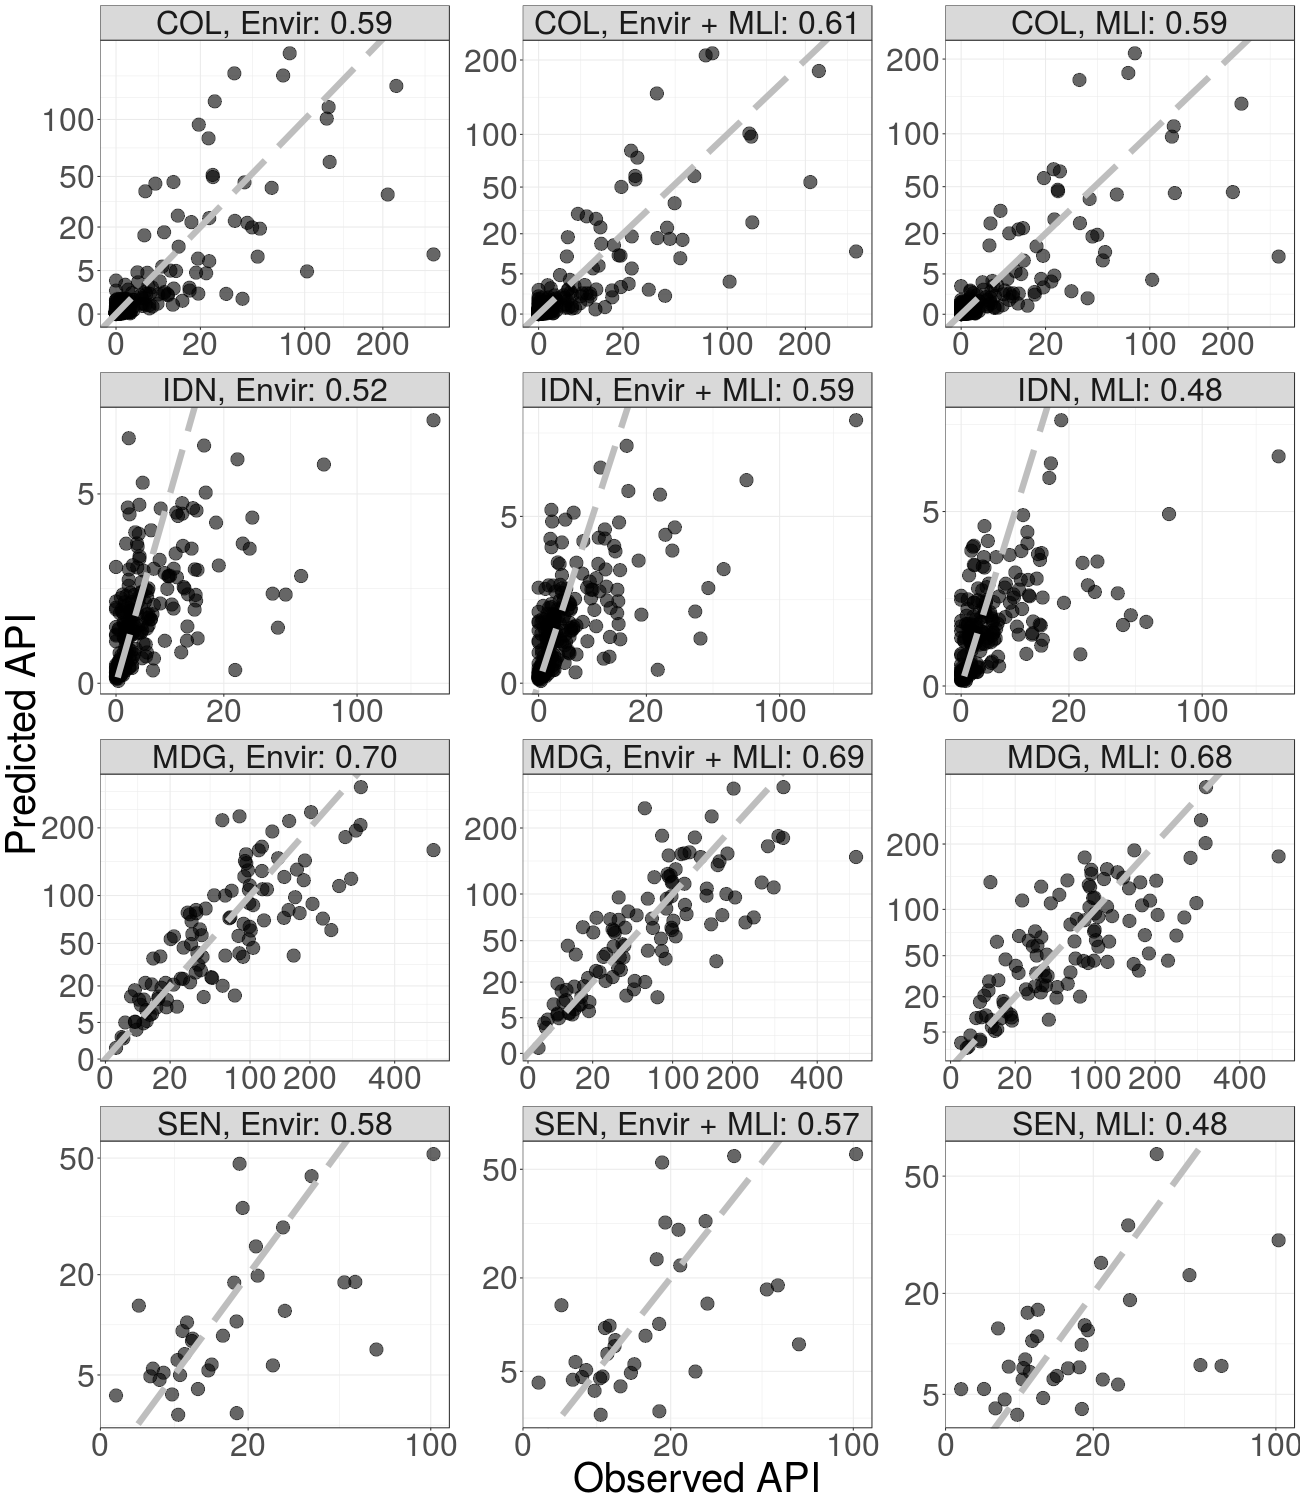
\includegraphics[width=\textwidth]{figs/cv1_l_scatter.png}
\caption{
  Observed data against predictions for random cross-validation hold-out samples on a square root transformed scale.
}
\label{f:scatter1}
\end{figure}


\begin{figure}
  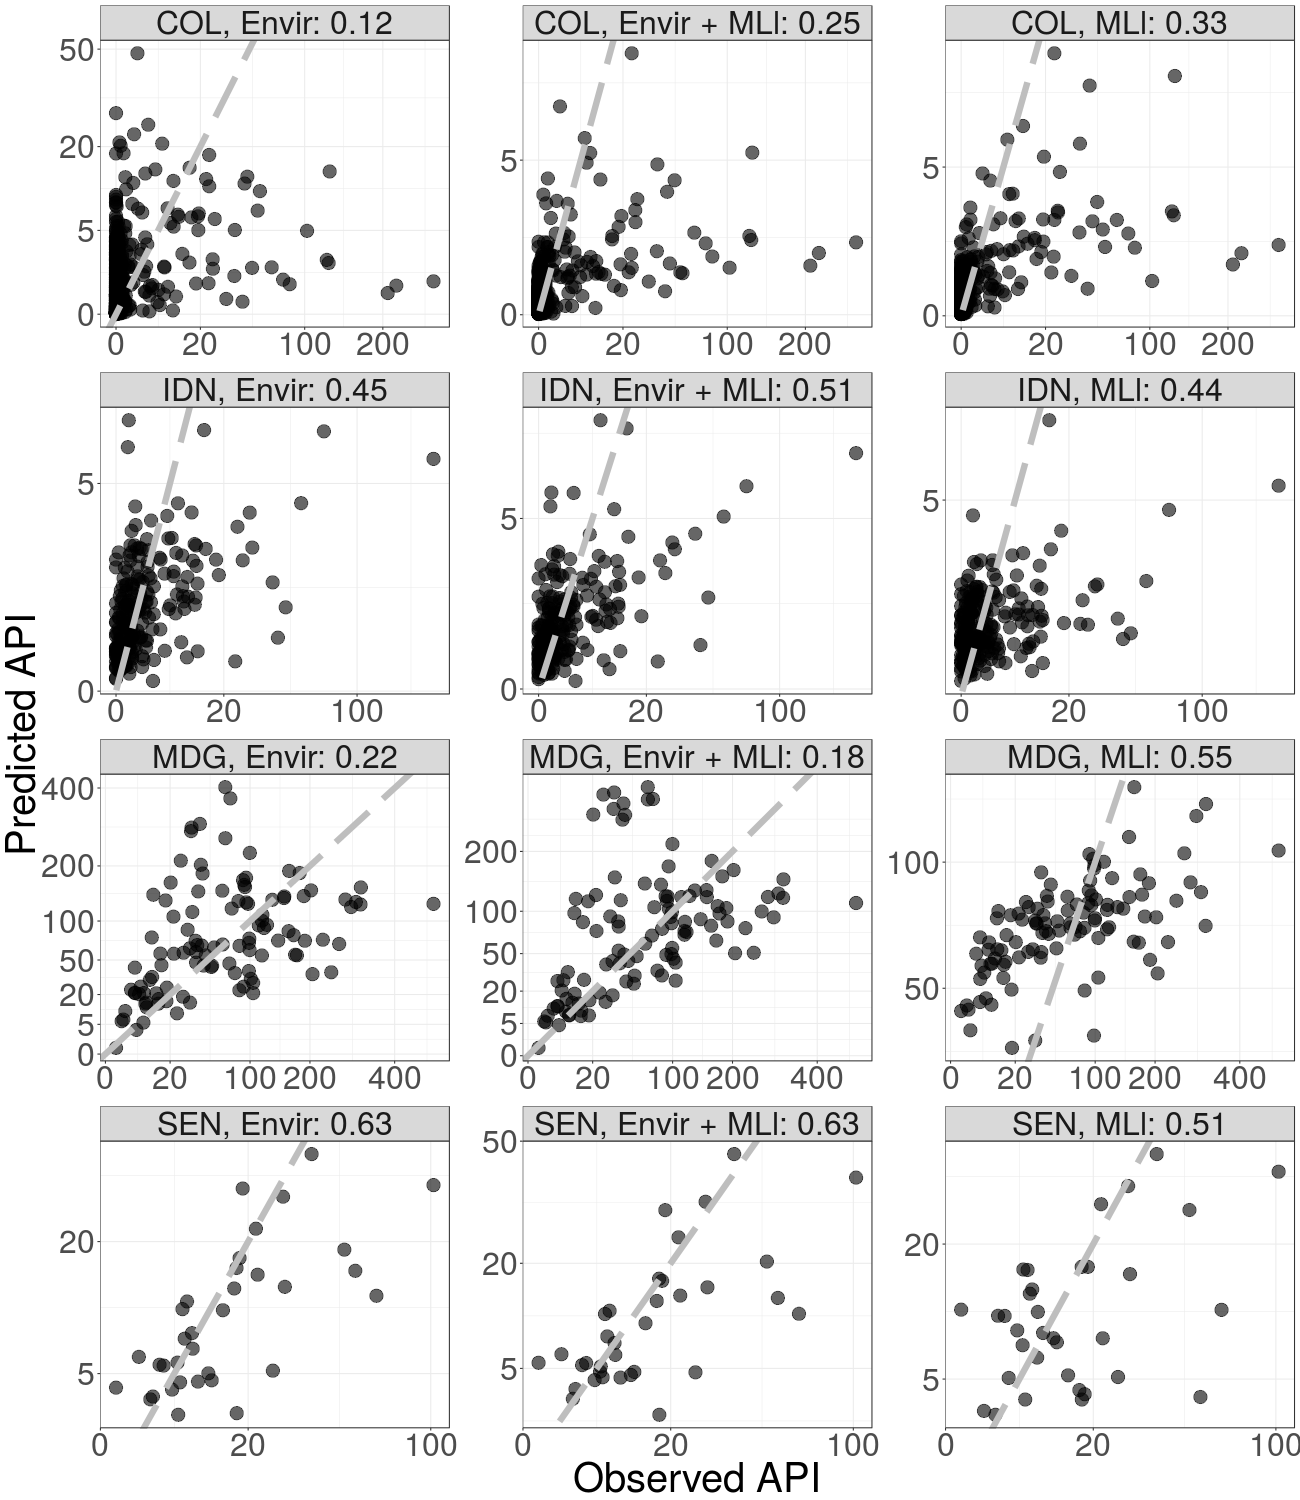
\includegraphics[width=\textwidth]{figs/cv2_l_scatter.png}
\caption{
  Observed data against predictions for spatial cross-validation hold-out samples on a square root transformed scale.
}
\label{f:scatter2}
\end{figure}

Figures~\ref{f:scatter1} shows scatter plots of the model performance under random cross-validation for experiment \emph{i}.
Figures~\ref{f:scatter2} shows scatter plots of the model performance under spatial cross-validation for experiment \emph{i}.
It can be seen that without environmental covariates, the models in Madagascar fail to predict very high or very low values correctly.
Figure~\ref{f:map} shows the input data and spatially out-of-sample predictions of the Enviro model and ML\textsubscript{l} model in Colombia.



Table \ref{t:results2} gives the correlation between observed and held out data (under random and spatially cross-validation) for experiment \emph{ii} (models Enviro, ML\textsubscript{g} and ML\textsubscript{l} + ML\textsubscript{g}).
In six cases, Enviro is the best or tied best performing model.
The ML\textsubscript{g} model is never the best performing model and only outpeforms Enviro in one case (spatial cross-validation in Madagascar).
In two cases ML\textsubscript{l} + ML\textsubscript{g} is the best performing model (spatial Colombia and spatial Madagascar).
Comparing across Tables \ref{t:results} and \ref{t:results2} we can see that ML\textsubscript{g} outpeforms ML\textsubscript{l} once (spatial cross-validation in Senegal).
In only two cases (Spatial Senegal and Spatial Indonesia) does ML\textsubscript{l} + ML\textsubscript{g} outperform ML\textsubscript{l}.



\begin{figure}[t!]
\centering
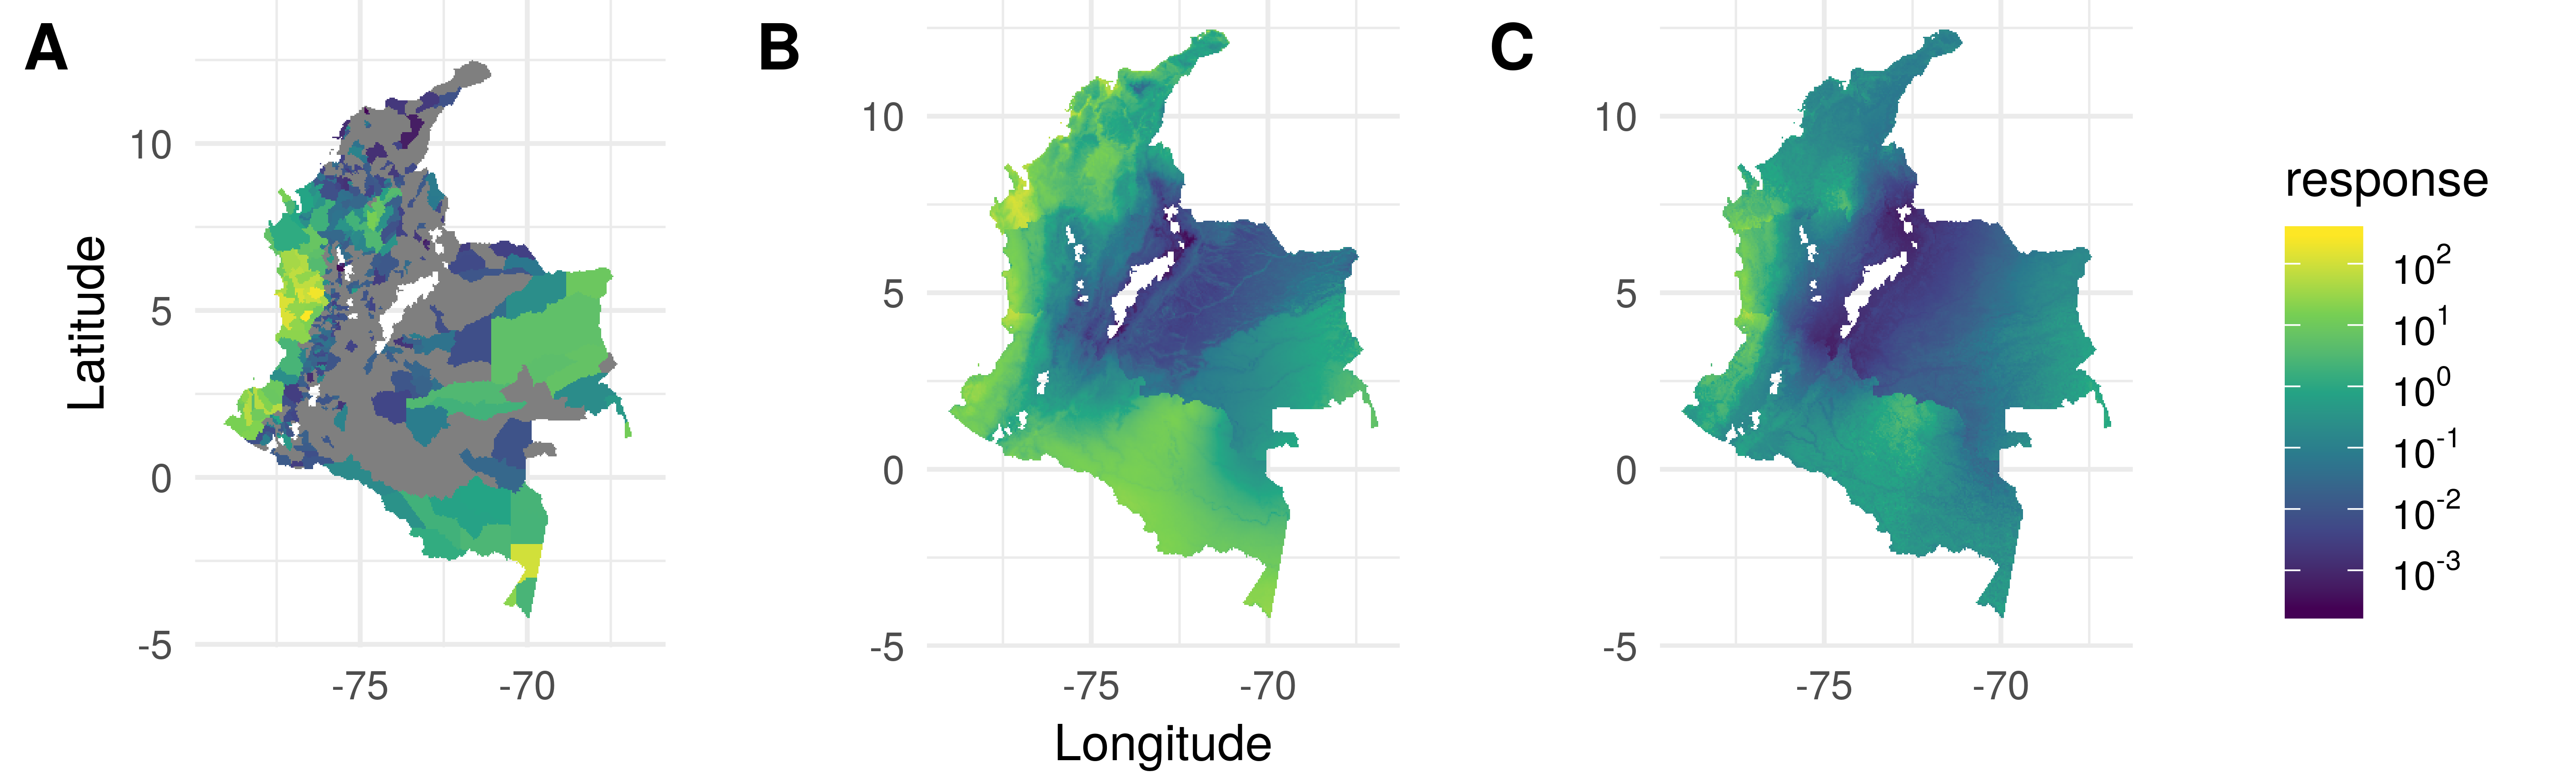
\includegraphics[width = 1\textwidth]{figs/col_comparison_map.png} %\caption{Indonesia spatial crossvalidation} 
\caption{
  A) Observed data for Colombia (grey for zero incidence). B) Out-of-sample predictions for the spatial cross-validation, environmental covariates only model. C) Out-of-sample predictions for the spatial cross-validation, local machine learning only model. For each cross-validation fold, predictions are made for the held out data which are then combined to make a single surface.
}
\label{f:map}
\end{figure}

Table~\ref{t:coverage} shows the out-of-sample coverage of the 80\% credible intervals for all models, countries and cross-validation schemes.
The coverage in Colombia is very poor with no models achieving a coverage above 0.4.
The coverage is acceptable in the other three countries with most values lying between 0.7 and 0.9.
Overall there is a general tendancy for models to be slightly over confident.

We can examine the relationship between the RMSE of the machine learning models to their fitted regression coefficients (weights).
These values are given in Table~\ref{t:mlresults}.
In all five sets of machine learning models (four sets trained on local data and one set trained on local data), Random Forest performs the best.
We have not forced $\beta_i > 0$ but we have set the priors for these coefficients with a positive mean.
In nearly all cases the fitted values are positive.
If the prevalence data and incidence data are not biased relative to each other we would expect the models with the lowest RMSE to also have the biggest regression coefficient.
This occurs in three cases where Random Forest has the lowest RMSE and the biggest coefficient.
In a further two cases, Random Forest has the lowest RMSE but GBM has the highest coefficient.
The predictions from Random Forest and GBM are highly correlated in part because they both perform well and in part because they are both tree based models.
Finally, it can be seen that the relationship between RMSE and regression coefficients was much weaker in Indonesia.
For the models trained on local data a neural network has the highest fitted coefficient while for the models trained on global data an elastic net has the highest fitted coefficient.





%\begin{table}[h!]
%\caption{Pearson correlations between observed and predicted values. }
%\centering
%\begin{tabular}{llrrrr}
%Cross-validation scheme & Country &  Covariates &  ML\textsubscript{l} &  ML\textsubscript{g} & ML\textsubscript{l} + ML\textsubscript{g} \\
%\hline 
% Random &  Colombia & \textbf{0.59} & \textbf{0.59} &  0.58 & 0.56 \\
% Random &  Madagascar &  0.70 &  \textbf{0.73} &   0.70 & 0.71 \\
% Random &  Senegal &  \textbf{0.58} &  0.51 &  0.30 & 0.08 \\
% Random &  Indonesia &  \textbf{0.52} &  0.48 &  0.46 & 0.32 \\
% Spatial &  Colombia &  0.12 &  0.33 &  0.18 & \textbf{0.34}\\
% Spatial &  Madagascar &  0.22 &  \textbf{0.66} &  0.63 & 0.60\\
% Spatial &  Senegal &  \textbf{0.63} &  0.27 &  0.36 & 0.35 \\
% Spatial &  Indonesia &  \textbf{0.45} &  0.44 &  0.41 & \textbf{0.45} \\
%\end{tabular}
%\label{t:results}
%\end{table}

% to do table of coverage.





\begin{table}[t!]
\caption{Pearson correlations between observed and predicted values. }
\centering
\begin{tabular}{llrrrr}
Country &  Cross-validation & Enviro &   ML\textsubscript{g} & ML\textsubscript{l} + ML\textsubscript{g} \\
\hline 
 Colombia & Random &  \textbf{0.59} &0.55 & 0.58 \\
 Colombia &  Spatial &  0.12 &  0.12 & \textbf{0.33}\\
 Indonesia &  Random &  \textbf{0.52} & 0.32 & 0.46 \\
 Indonesia &  Spatial &  0.45 & 0.41 & 0.45 \\
 Madagascar &  Random &  \textbf{0.70} &  0.67 & 0.68 \\
 Madagascar &  Spatial &  0.22 &  0.51 & \textbf{0.55}\\
 Senegal &  Random &  \textbf{0.58} &  0.50 & 0.49 \\
 Senegal &  Spatial &   \textbf{0.63} & 0.55 & 0.52 \\

\end{tabular}
\label{t:results2}
\end{table}



\begin{table}[t!]
\caption{Covarage of 80\% credible intervals. Values outside 0.7--0.9 are shown in bold.}
\centering
\begin{tabular}{llrrrrr}
Country &  CV & Enviro & ML\textsubscript{l} &  Enviro + ML\textsubscript{l} & ML\textsubscript{g} & ML\textsubscript{l} + ML\textsubscript{g} \\
\hline 
 Colombia & Random & \textbf{0.28} & \textbf{0.28} & \textbf{0.29} & \textbf{0.28} & \textbf{0.30} \\
 Colombia &  Spatial & \textbf{0.30} & \textbf{0.33}  & \textbf{0.33} & \textbf{0.33} & \textbf{0.34}  \\
 Indonesia & Random &0.80 & 0.81& 0.78& 0.79& 0.77  \\
 Indonesia & Spatial & 0.80 & 0.78& 0.78& 0.76& 0.75  \\
 Madagascar &  Random & 0.80 & 0.77& 0.75& 0.77& 0.76 \\
 Madagascar & Spatial & \textbf{0.65} & 0.74& 0.70& 0.75 & 0.76   \\
 Senegal & Random &0.79 & 0.79& 0.79& 0.79& 0.82 \\
 Senegal & Spatial & 0.85 & \textbf{0.91}& 0.85& \textbf{0.94} & 0.85  \\
\end{tabular}
\label{t:coverage}
\end{table}




\begin{table}[t!]
\caption{Machine learning model results and fitted parameters (i.e.\thinspace model weights) of the machine learning predictions only models (local only and global only). }
\centering
\small
\begin{tabular}{ll|rr|rr}
     Country          & Model &      RMSE\textsubscript{l} & $\beta_l$ & RMSE\textsubscript{g} & $\beta_g$ \\ \hline
Colombia & RF & \textbf{0.068} & 0.625 &  \textbf{0.169} & 0.180\\
Colombia & GBM & 0.073 & \textbf{0.952} & 0.178& -0.218  \\
Colombia & enet & 0.070 & 0.219 &0.233 & 0.183 \\
Colombia & nnet & 0.070 & 0.129 &0.220 & 0.527 \\
Colombia & ppr & 0.070 & 0.667 & 0.205 &  \textbf{0.546}\vspace{0.3cm}\\
Indonesia & RF& \textbf{0.081} & 0.447 & \textbf{0.169} & 0.178\\
Indonesia & GBM & 0.085 & 0.357 & 0.178& 0.289 \\
Indonesia & enet & 0.091 & 0.303 &0.233 & \textbf{0.526} \\
Indonesia & nnet & 0.089 & \textbf{0.506} &0.220 & 0.316 \\
Indonesia & ppr & 0.089 & 0.364 & 0.205 &  0.089\vspace{0.3cm}\\
Madagascar & RF & \textbf{0.100} & 0.538 &  \textbf{0.169} & \textbf{0.529}\\
Madagascar & GBM & 0.105 & \textbf{0.570} & 0.178& 0.432 \\
Madagascar & enet & 0.116 & 0.301 &0.233 & 0.262 \\
Madagascar & nnet & 0.113 & 0.033 &0.220 & 0.364 \\
Madagascar & ppr & 0.109 & 0.469 & 0.205 &  0.403\vspace{0.3cm}\\ 
Senegal & RF & \textbf{0.092} & \textbf{0.339} & \textbf{0.169} & \textbf{0.425} \\
Senegal & GBM & 0.099 & 0.261& 0.178& 0.408 \\
Senegal & enet& 0.103 & 0.344  &0.233 & 0.205 \\
Senegal & nnet & 0.099 & 0.254 &0.220 & 0.190 \\
Senegal & ppr & 0.098 & 0.268& 0.205 &  0.126\\


\end{tabular}
\label{t:mlresults}
\end{table}







%\begin{table}
%\caption{Fitted regression parameters of the environmental and machine learning covariates for thee models: just environmental variables, just local machine learning models and the combination of the two.}
%\centering
%\tiny
%\begin{tabular}{ll|rrr}
%Country    & Variable &  $\beta_{enviro}$   & $\beta_l$ & $\beta_{enviro+l}$\\ \hline
%Madagascar & LST mean & 0.17 &  &  -0.01\\
%Madagascar & EVI & 0.32 &  & -0.04 \\
%Madagascar & TSI & 0.42 &  &0.06  \\
%Madagascar & access & 0.34 &  &0.00  \\
%Madagascar & Elev & -0.14 &  & 0.00\\ 
%Madagascar & LST sd & -0.78 &  &-0.04  \\
%Madagascar & VIIRS & -0.1 &  &-0.52  \\
%Madagascar & TCW & -0.22 &  & -0.06\\ 
%Madagascar & RF &  & 0.29 &  0.01\\
%Madagascar & GBM &  & 0.52 & 0.25 \\
%Madagascar & enet &  & 0.31 &0.09  \\
%Madagascar & nnet &  & 0.43 &0.14  \\
%Madagascar & ppr &  & 0.49 & 0.22\vspace{0.2cm}\\ 
%Colombia & LST mean &-0.12  &  & -0.22\\
%Colombia & EVI &  -0.08&  & 0.17\\
%Colombia & TSI &  0.54&  & -0.06\\
%Colombia & access &  0.35&  &0.00 \\
%Colombia & Elev &  0.47&  & 0.00\\
%Colombia & LST sd & -0.11 &  & -0.10\\
%Colombia & VIIRS & 0.24 &  & 0.01\\
%Colombia & TCW &  0.21&  & 0.00\\
%Colombia & RF &  & 0.36 & -0.18\\
%Colombia & GBM &  & 0.54 & 0.26\\
%Colombia & enet &  & 0.32 & -0.34\\
%Colombia & nnet &  &0.33  & -0.09\\
%Colombia & ppr &  & 0.54 & 0.01\vspace{0.2cm}\\
%Senegal & LST mean &-0.04  &  &-0.02\\
%Senegal & EVI &  0.33&  & 0.30\\
%Senegal & TSI &  -0.58&  &  -0.59\\
%Senegal & access & -0.03 &  &  -0.05\\
%Senegal & Elev &  0.42&  &0.37\\ 
%Senegal & LST sd &  0.21&  & 0.10 \\
%Senegal & VIIRS &  0.13&  &  0.13\\
%Senegal & TCW & 0.08 &  &-0.01\\ 
%Senegal & RF &  & 0.34 &  0.20\\
%Senegal & GBM &  &  0.28& 0.05\\
%Senegal & enet &  &  0.27&  -0.05\\
%Senegal & nnet &  & 0.29 &-0.09 \\
%Senegal & ppr &  &  0.35& 0.25\vspace{0.2cm}\\
%Indonesia & LST mean & -0.32 &  &-0.34\\
%Indonesia & EVI &  0.49&  & 0.36\\
%Indonesia & TSI &  0.58&  &0.52\\
%Indonesia & access &0.33 &  & 0.06 \\
%Indonesia & Elev& -0.06&  &-0.13\\ 
%Indonesia & LST sd & -0.23 &  & -0.33\\
%Indonesia & VIIRS &  -0.12&  & 0.03\\
%Indonesia & TCW& 0.12 &  &0.10\\ 
%Indonesia & RF &  & 0.32 & 0.06\\
%Indonesia & GBM &  &  0.38&0.03\\
%Indonesia & enet &  &  0.49&  0.56\\
%Indonesia & nnet &  &  0.36&  0.18\\
%Indonesia & ppr &  &  0.45& 0.32\\
%
%
%
%\end{tabular}
%\label{t:mlresults2}
%\end{table}
%


\section{Discussion}


Overall, experiment \emph{i} suggest that using predictions from machine learning models trained on local prevalence points provides more accurate predictions than using environmental covariates when fitting disaggregation models of malaria incidence.
This increased performance comes despite the data being on different scales, the data being measurements of different aspects of malaria transmission and despite the imperfect model we have used to translate between the two scales.
However, there is no clear best model between ML\textsubscript{l} and Enviro + ML\textsubscript{l}.
Therefore, when using these methods, both of these models should be fitted and the most predictive model selected for a given dataset.
Furthermore, many of the performance improvements are rather marginal. 
However, in a few cases such as Colombia and Madagascar under spatial cross-validation the performance boost is large.
For example, using just environmental covariates in Madagascar under spatial cross-validation gives a correlation between observed and predicted data of 0.22.
Such a model would be unusable for any applied or policy work.
In contrast, using the predictions from the machine learning models trained on local data gives a correlation value of 0.55, which while still relatively poor is possibly a useful model.

As expected, the model performance was generally worse under spatial cross-validation than under random cross-validation.
This implies that the models are still relying heavily on the spatial Gaussian random field.
Furthermore, the difference between random and spatial cross-validation is usually bigger than the difference between different models.
This suggests that better data coverage is more important than which specific model is used.


% this method is an improvement
% still reliant on spatial field

% allows broad suite of covariates

% sum to one stacking

% global ml models, local experts

Overall, the models fitted using predictions from machine learning models trained on the global database of prevalence point-surveys were less good than those using either environmental data alone or than those using predictions from machine learning models trained on local data.
This in itself is not particularly surprising.
However, it does indicate that continental scale models should consider using a mosaic of locally trained machine learning models for example.
What is more surprising is that using both the ML\textsubscript{l} and ML\textsubscript{g} covariates together did not improve performance given that this approach of creating diverse predictions is a core element of stacking methodology.

While the approach presented here is related to stacking, it differs in that we have not constrained the regression parameters to be positive nor included a sum-to-one constraint i.e.\thinspace the result is not simply a weighted average of the level zero model predictions.
We did not include these constraints because the base models and the meta model are trained on response data on different scales.
However, given our priors, nearly all the fitted regression coefficients in models with only machine learning predictions were positive.
Therefore, in practice these models are working in a way similar to standard stacking.
However, the coefficients certainly do not sum to one, and fitted intercepts are very small to account for this.


Due to the low power of typical aggregated incidence datasets, previous analyses using disaggregation regression used a small number of covariates \citep{sturrock2014fine}.
However, as models such as Random Forest and elastic net can robustly handle high dimensional data, future work could include many more covariates in the machine learning models, potentially increasing predictive performance.
However, to make comparisons more easy, here we have used the same environmental covariates in the machine learning models and in the Enviro disaggregation regression models.



\section{Conclusions}

Overall we find that including predictions from machine learning models trained on prevalence point-surveys can improve the performance of disaggregation regression models for malaria incidence relative to using raw environmental covariates.
This extra modelling step can be seen as finding useful, non-linear transformations of the raw environmental covariates.
This view is important for understanding how the model will predict in areas with no incidence data; in this situation the Gaussian random field has no effect and predictions are driven by this non-linear transformation of the raw environmental covariates.
Training the machine learning models on local data (i.e. prevalence data from the same country or region as the incidence data) gave much better performance than when training the machine learning models on the full, global, dataset of prevalence point-surveys.
As more countries start providing timely and accurate routine surveillance data of malaria cases disaggregation regression may become more popular.
We have here presented a method for improving these models by using ancillary, prevalence point-survey data.



\section*{Acknowledgments}
The authors acknowledge the National Malaria Control Programme of Madagascar for sharing their routine case data for this analysis.

\bibliography{Malaria} 
%\bibliographystyle{unsrt}
%\bibliographystyle{apalike}




\end{document}









